\documentclass[a4paper,spanish]{article}

\usepackage{url}
\usepackage{verbatim}

\usepackage[activeacute]{babel}
\usepackage{fancyhdr}
\usepackage{ecarat}
\usepackage{graphicx}
%\usepackage{amssymb}
\usepackage{amssymb,amsmath}
%\usepackage[all]{xy}
\usepackage{graphicx}
\usepackage{listings}
%\usepackage{pseudocode}
\usepackage[utf8]{inputenc}
%\usepackage{wrapfig}
\usepackage{lastpage}
\usepackage{multicol}
\usepackage{url}
\usepackage{color}
\usepackage{array}
\usepackage{url}
\usepackage{listings}
\usepackage{sverb}

\graphicspath{
{./images/}
}

\usepackage{xifthen}% provides \isempty test
%~ \usepackage{ulem}%para subrayados
\usepackage{dashrule}%para subrayados

%~ \usepackage{relacion}

\oddsidemargin 0in
\textwidth 6.5in
\topmargin 0in
\addtolength{\topmargin}{-.4in}
\addtolength{\leftmargin}{-.5in}
\textheight 10in
\parskip=1ex
\pagestyle{fancy}
\newcommand{\real}{\hbox{\bf R}}
\newcommand{\prima}{^{\prime}}
\newcommand{\tab}{\hspace*{1cm}}
%Cosas que se usan en el enunciado
% \parindent = 0 pt
% \parskip = 11 pt

\usepackage{a4wide}
\newcommand{\erf}{\hbox{erf}}
\newcommand\abs[1]{\ensuremath{\left| {#1} \right|}}
%~ \addtolength{\textheight}{1cm}

\lstdefinelanguage{Smalltalk}{ 
	morekeywords={true,false,self,super,nil}, 
	sensitive=true, 
	morecomment=[s]{"}{"}, 
	morestring=[d]', 
	style=SmalltalkStyle 
} 
\lstdefinestyle{SmalltalkStyle}{ 
	literate={:=}{{$\gets$}}1{^}{{$\uparrow$}}1 
} 
\lstset {%
     language=Smalltalk,
     frame=l,
     framerule=1pt,
     aboveskip=1em,
     framextopmargin=3pt,
     framexbottommargin=3pt,
     framexleftmargin=0.4cm,
     framesep=0pt,
     rulesep=.4pt,
     %~ backgroundcolor=\color{gris95},
     rulesepcolor=\color{red},
     tabsize=4,
     %
     stringstyle=\sffamily,
     showstringspaces = false,
     basicstyle=\footnotesize\sffamily,
     identifierstyle=,
     commentstyle=\em, %\sffamily\color{gris50},
     keywordstyle=\bfseries,
     commentstyle=\scriptsize\sffamily,
     breaklines=true,
     breakatwhitespace=true,
     morekeywords={setof},
   }

\usepackage{longtable}


\hyphenation{ob-te-ner}

\begin{document}

\materia{Herramientas computacionales en Neurociencias}
\titulo{Trabajo Pr\'{a}ctico}
\subtitulo{Pr\'actica 6 - Spike Sorting}
\abst{s }
\grupo{}
\claves{}
\integrante{Daniel J. Foguelman}{667/06}{dj.foguleman@gmail.com}


%\lhead{\parbox{7.4cm}{\small TP \textsc{Teor\'{i}a de Lenguajes}}}

\cfoot{$\thepage$ de \pageref{LastPage}}

\thispagestyle{empty}

\maketitle




%\tableofcontents

%\pagebreak

\section{Introducci'on}
\subsection{`? Por qu\'e Spike-Sorting?}

\subsection{Temas abarcados en la pr\'actica}

\subsection{Objetivos}

\section{Desarrollo}
\subsection{Datos, an\'alisis}
\subsection{Filtering}
\subsection{Feature an\'alisis}
\subsection{Clustering}


\section{La Pr\'actica}
\subsection{Problema 1}
En este problema se pide graficar un dataset que tiene la siguiente estructura:
\begin{tabular}{ c | c | c | c}
	spikes & cluster\_class & inspk & par \\
\end{tabular}

Y analizar la cantidad de neuronas que podr\'ian encontrarse en dichos datos.

Comenzamos trabajando sobre la variable spikes. Entendemos que estos datos ya se encuentran:
\begin{itemize}
	\item Filtrados
	\item Ya se ha hecho un trabajo de Spike detection (con Amplitude Threshold o alg\'un m\'etodo similar).  
\end{itemize}


El problema de Spike-Sorting, a grandes rasgos, trata de mapear un tren de spikes en m\'ultiples canales de medici\'on con el de una sola neurona. Las dificultades para distinguir cada neurona en particular puede deberse a:
\begin{itemize}
	\item Distintos canales miden la misma neurona desde distintos lugares y distancias, mostrando distintos valores. (Quin Quiroga cita Gold et al., 2006)
	\item La sincronizaci\'on inter-neuronal lleva a la superposici\'on de se\~nales. (Phase Synchronization).
	\item Mala elecci\'on de par\'ametros en los procesos de Detecci\'on de Spikes y de Features.
\end{itemize}

La pregunta que subyace de este an\'alisis ser\'ia entonces ¿cuantas neuronas podemos contar a partir de los datos que tenemos?
Sabemos que habr\'a al menos tantas neuronas como clases de features. ¿Pero cuantas m\'as habr\'a? ¿C\'omo distinguimos neuronas sincronizadas?

En la figura ~\ref{fig1} podemos observar cuatro features distintos, ¿cuantos otros features no son analizables a simple vista y precisan de un proceso m\'as sofisticado? 

Las preguntas que queremos responder utilizando alg\'un m\'etodo de Clustering entonces ser\'ian:
%%%% TODO: Reforzar preguntas FLOJO
\begin{itemize}
	\item Cada Feature corresponde al spike-train de\textbf{una} neurona o de varias? 
	\item Hemos distinguido \textbf{todos} los features? 
	\item Podemos encontrar se\~ales de otras neuronas en ellos?
\end{itemize}

Poniendolo en t\'erminos de data mining, podemos armar una partici\'on de las N observaciones en K clusters donde cada observaci\'on pertenece al cluster con media m\'as cercana.
Haciendo un an\'alisis meramente cuantitativo, podemos ver que para $N > K$, por el principio del palomar, dos observaciones pertenecer\'an al mismo cluster. Esto implica que por cada cluster, estaremos necesariamente encontrando se\~nales de varias neuronas, o bien sincronizadas, o bien que no pudimos separar en la etapa de filtrado o de detecci\'on de features.



%%%% TODO: Mejorar grafico.
\begin{figure}[htc]
	\centering
	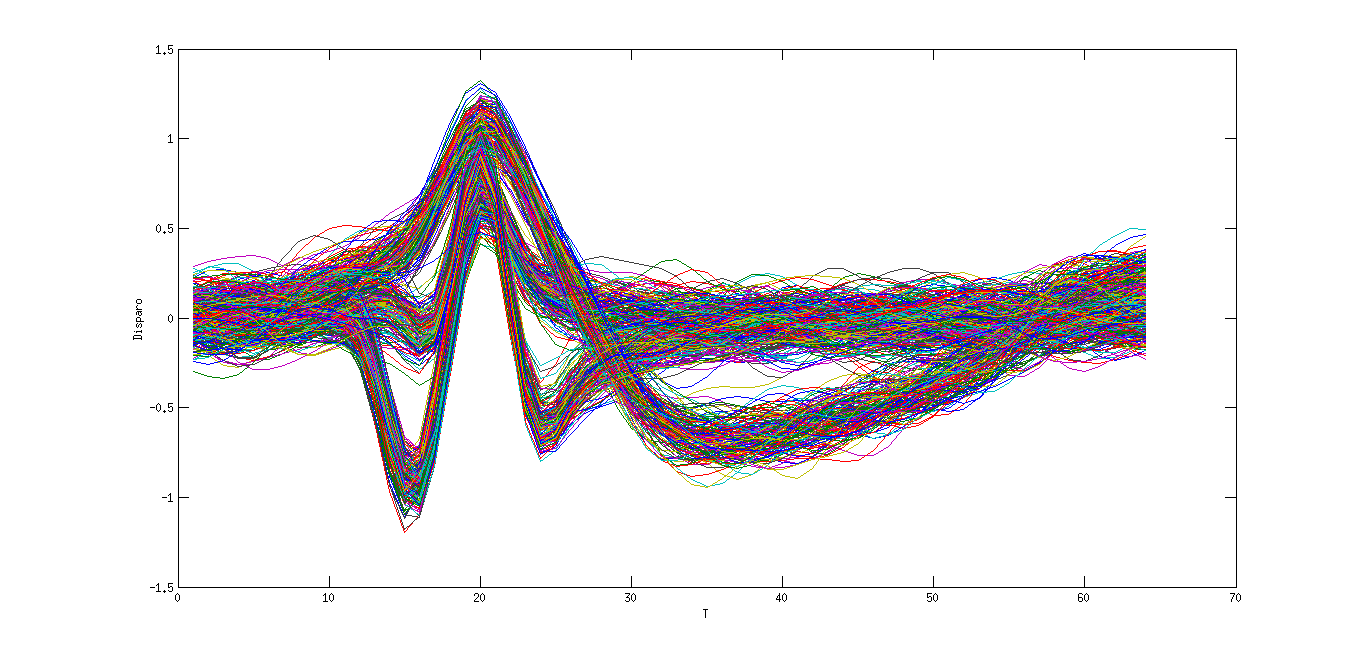
\includegraphics[width=1.0\textwidth]{imgs/spikes_data_1.png}
	\caption{Spikes por tiempo. Datos de data\_sim1.}
	\label{fig1}
\end{figure}


%%%% Aca hablo de lo importante de clasificar

%%% Classification is the task of learning a target function f that maps each attribute set x to one of the predefined class labels y.  The target function is also known informally as a classification model.  A classification model is useful for the following purposes.



Veamos qu\'e sucede aplicando el m\'etodo de K-Means a los datos dados:

%%%% TODO: Mejorar grafico.
\begin{figure}[htc]
	\centering
	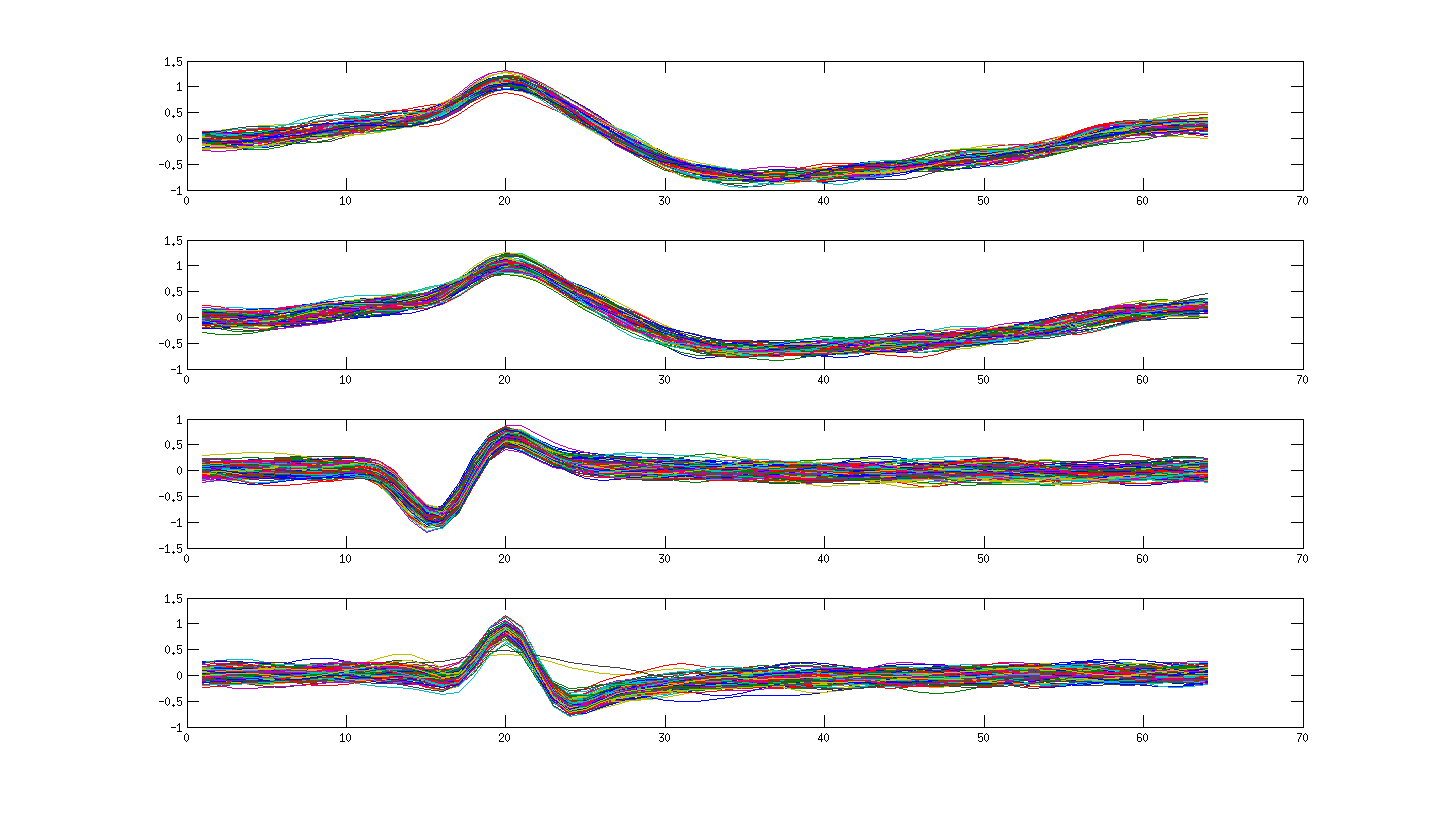
\includegraphics[width=1.0\textwidth]{imgs/clustering_4_data_1.png}
	\caption{Clustering en cuatro clases los datos en data\_sim1.}
	\label{fig2}
\end{figure}


%%%% Aca hablo de K-Means, propiedades, etc.
El algor\'itmo realiza una categorizaci\'on, en un espacio de categor\'ias fijo, agrupando las observaciones seg\'un su media. Cada observaci\'on pertenecer\'a a un cluster tal que se minimice las sumas de las medias de cada cluster.


%%%% Hablo de Confusion matrix
%%%% Misclassification error, como estimarlo, cuan malo es



\subsection{Problema 2}

Amplitude Threshold + Spike Alignation

Los datos que se presentan a continuaci\'on, son mediciones extracelulares filtradas. Se observaron 60 segundos de grabaci\'on extracelular con un Sample Rate de 24khz.
Desconocemos la relaci\'on Se\~nal Ruido pero podemos observar, realizando un histograma de los datos cuales son las frecuencias con mayor aparici\'on. Si consideramos que el ruido presente tiene las siguientes caracteristicas:

\begin{itemize}
	\item La se\~al de ruido se encuentra en voltajes m\'as bajos que los spikes.
	\item Hay una relaci\'on se\~nal ruido desfavorable. (Hay menos spikes que ruido).
\end{itemize}

Podemos entonces filtrar las se\~ales m\'as bajas que cierto threshold. El c\'omo determinar el threshold ser\'a lo que influya en:

\begin{enumerate}[a.]
	\item Falsos positivos por un threshold muy bajo (Error de tipo I).
	\item No encontrar todos los spikes  por un threshold muy alto (Error de tipo II).
\end{enumerate}


Observando los datos crudos no obtenemos demasiada intuici\'on del problema.

\begin{figure}[htc]
	\centering
	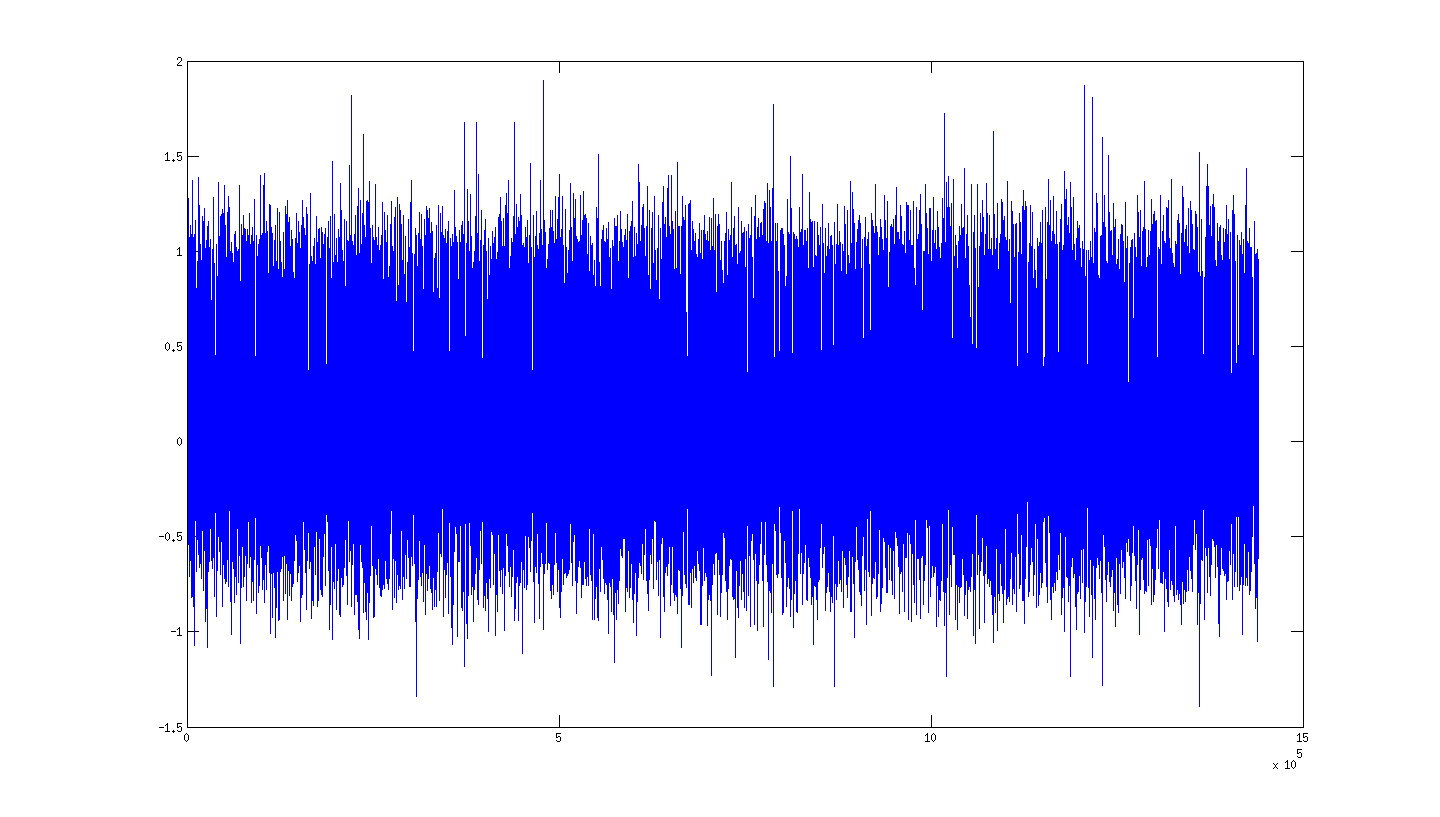
\includegraphics[width=1.0\textwidth]{imgs/raw_cont_data.png}
	\caption{Datos crudos en cont\_data, dataset.}
	\label{fig3}
\end{figure}


En la \ref{fig4} podemos observar que la frecuencia muestral de los voltajes entre 0.25 y 2 baja. Buscaremos estos valores y filtraremos por amplitud nuestros datos.
\begin{figure}[htc]
	\centering
	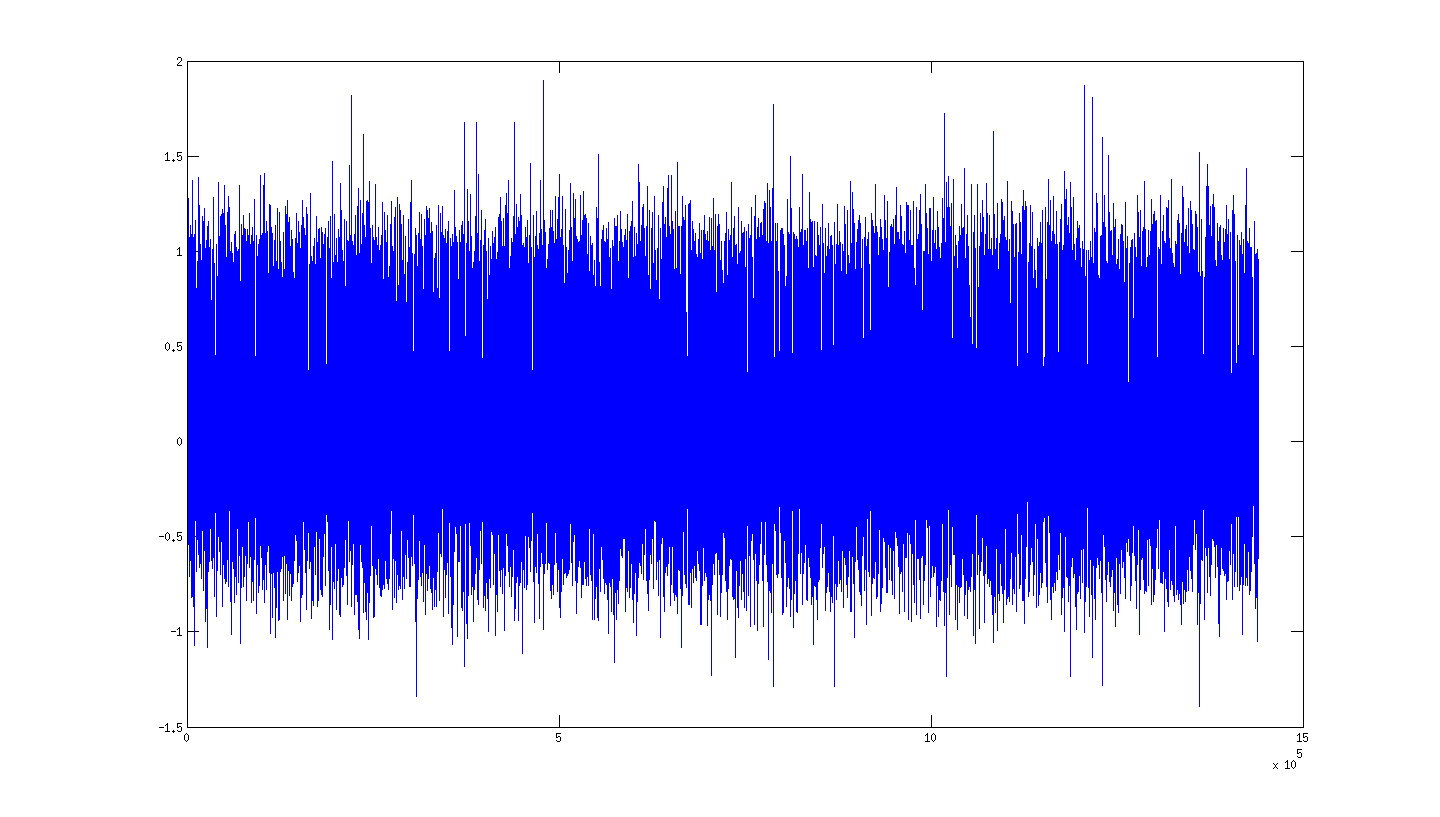
\includegraphics[width=1.0\textwidth]{imgs/raw_cont_data.png}
	\caption{Histograma contdata\sim2}
	\label{fig4}
\end{figure}


Implementando un algoritmo sencillo para el thresholding y alineaci\'on de los spikes, se recorre un set de datos a ventana fija  buscando un m\'aximo local. Utilizando este m\'aximo se recortar\'a la se\~nal en un entorno alrededor del punto. Considerando una duraci\'on t\'ipica por spike de entre 2 y 3 ms. por spike se toma una ventana de 2.5 ms., considerando que el Sample Rate es de 24khz, se toma una ventana de tama\~o $ fraq{2.5 * 24000}{1000}$ asim\'etrica, es decir que los samples que van desde el 0 hasta el 24 son los previos al m\'aximo local y los siguientes 36 se encontrar\'an n la cola del spike. Entonces lo que precede al m\'aximo local del spike es el primer ms. y lo que sigue detras los \'ultimos 1.5 ms. grabados. Luego de la detecci\'on del spike, se guarda en una matriz. Todas las muestras tendr\'an el mismo tama\~o (60 samples) y estar\'ian centradas.

Observaremos luego que no pudieron ser centradas con un algor\'itmo tan simple.

La utilizaci\'on del script es sencilla, primero cargamos los datos y luego invocamos la funci\'on.

\begin{verbatim}
>> d = load('contdata_sim2.mat');
>> data = spike_detect(d.data, d.par.sr, 1, 1440000, true); 
\end{verbatim}

Los parametros con los que la invocamos se detallan a continuaci\'on:
\begin{itemize}
	\item La data cruda
	\item El sample rate
	\item A partir de qu\'e muestra.
	\item Hasta qu\'e muestra.
	\item Utilizar 3Std como threshold o el de la mediana propuesto por Quian Quiroga 2004.
\end{itemize}

\begin{figure}[htc]
	\centering
	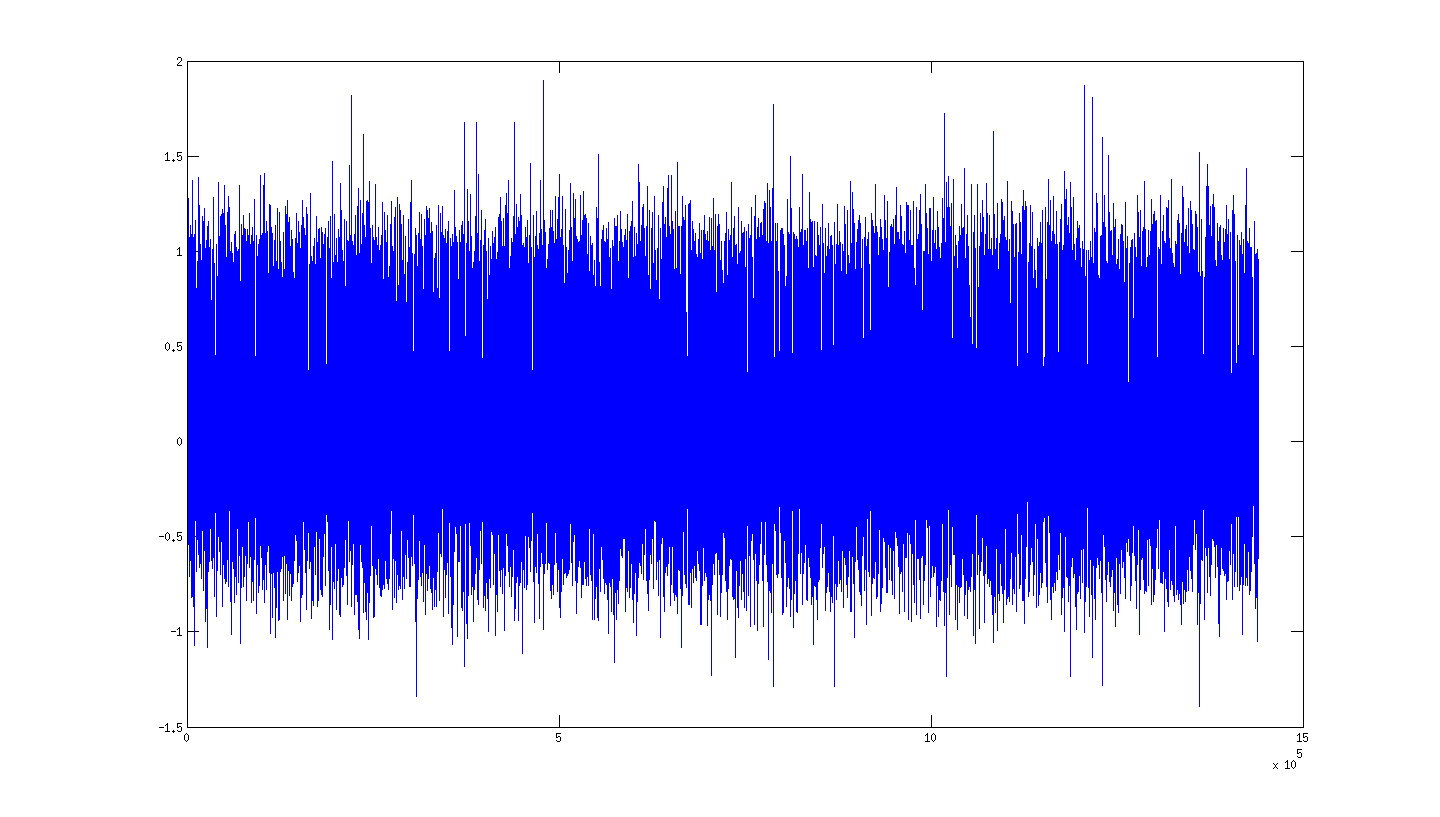
\includegraphics[width=1.0\textwidth]{imgs/raw_cont_data.png}
	\caption{Histograma contdata\sim2}
	\label{fig5}
\end{figure}

\begin{verbatim}
>> graphic_wavelforms(data, kmeans(data, 2), 2);

\end{verbatim}

\end{document}
